Fig.\ref{fig:v} upper panel Shows the cross correlation between 
the reconstructed velocity field $\hat v_{z,ns}$ and the real velocity field $v_z$, at redshift 1 and 2. 

At this point, all the manipulation and calculation on $\delta(\bm{k})$ are independent over different $\bm{k}$, 
therefore, the cross-correlation closely resembles the substraction we perform. 

Just one interesting thing to notice is that although the foreground at z=2 is stronger, 
the non-linear effects are weaker.  
So we still can obtain correlations at $k\parallel \lesssim 0.1$ from the seriously suppressed density contrast. 

Fig.\ref{fig:r} shows the cross correlation between the reconstructed kSZ map 
$\hat\Theta_{ns}$ and real kSZ map $\Theta$ at redshift 1 and 2. 
There are two points to notice: 

(1) For both redshift, there are a considerable amount of correlation 
$r\gtrsim0.5$ for $l\gtrsim 1000$; 
and this correlation drops quickly for smalller l; 

(2) The obtained correlation at redshift 2 is better than redshift 1.

To explain the behavior of the cross correlation, we write Eq.(\ref{eq:ksz}) in Fourier space.

\begin{eqnarray}
    \Theta(\bm{k_\perp^{\prime}})\equiv&\Theta&(k_x^{\prime},k_y^{\prime},0)\propto\int d^3k\delta(\bm{k_\perp^{\prime}}-\bm{k_\perp},k_\parallel) v_z(\bm{k})\nonumber\\
    \xrightarrow[region]{linear}&\int& d^3k\delta(\bm{k_\perp^{\prime}}-\bm{k_\perp},k_\parallel)\delta(\bm{k})\frac{k_z}{k^2}\\
    =&\int&d^3lnk\delta(\bm{k_\perp^{\prime}}-\bm{k_\perp},k_\parallel)\delta(\bm{k})\frac{k_z^2k_xk_y}{k^2}\nonumber
    \end{eqnarray}

    We transform $dk\rightarrow dlnk$ 
    to show the contributions from different k scales.
    The strength of $|\delta(\bm{k})|$ with respect to k can be seen in Fig.\ref{fig:delta}

For small $k_\perp^\prime=l/\chi\sim 0.1$ h/Mpc:

Although $\frac{k_z^2k_xk_y}{k^2}$ favors larger k, both $\delta(\bm{k_\perp^{\prime}}-\bm{k_\perp},k_\parallel)$  
reach peak at $k\sim 0.1 h/Mpc$.
and this makes a sufficient amount of contributions to the final integrated $\Theta$. 
On the other hand, the fields after foreground substraction lack the part from 
small $k_z$, which caused the null correlation.

For large $k_\perp^\prime\sim 1$h/Mpc:

$\delta(\bm{k_\perp^{\prime}}-\bm{k_\perp},k_\parallel)$ and $\delta(\bm{k})$ 
no longer reach peak at similar points.  
$\delta(\bm{k_\perp^{\prime}}-\bm{k_\perp},k_\parallel)\delta(\bm{k})$ 
has similar value for $k\sim 0.1$ h/Mpc and $k\sim 1$ h/Mpc, 
while $\frac{k_z^2k_xk_y}{k^2}$ weights the later a hundred times heavier.
Therefore, the importance of small k modes is attenuated.

Fig.\ref{fig:delta} is a set of plots that helps understand the behavior.

The reason why the correlation on redshift 2 is better is that 
the density contrast at redshift 1 is sharper than redshift 2, 
which exaggerates the contribution from small scales.

Although performs badly at small l, the reconstructed kSZ signal $\hat \Theta_{ns}$ 
from 21cm density field shall still be able to give us reasonable S/N in real applications  
, because most kSZ signals that can be distinguished come from $l\gtrsim 1000$, when primary CMB gradually dies out. 

However, based on the analysis above, 
we will expect a further improvement on cross correlation 
if we recover the small k modes lost in noises. 
In next section, we provide a method to achieve the goal.


\begin{figure}[tbp]
\begin{center}
\includegraphics[width=0.48\textwidth]{compare_powv2d_z1z2.eps}
\end{center}
\vspace{-0.7cm}
\caption{(Top) The cross correlation r between $P_{v_z}$ and 
    $P_{\hat v_z^{fs}}$ calculated from foreground substracted field $\delta_{fs}$; 
    (Bottom) The cross correlation between $P_{v_z}$ and $P_{\hat v_z^{tide}}$ calculated from $\hat \kappa_c$. 
The contour line indicates $k^3 P(k)$.
}
\label{fig:v}
\end{figure}
